\chapter{Data Analysis} \label{ch:analysis}
The analysis of the data involved extrapolating the available spectra and using the results from the fit to calculate the transverse energy and particle multiplicities corresponding to each spectrum. 
\section{Extrapolation of Spectra}
The available spectra were limited to a range of transverse momenta ranging from ..... to ...... in the lower-energy less-central collisions to  ..... to ....... in the higher-energy more-central collisions. To account for the missing transverse energy found from using just the available data histograms,
\subsection{Boltzmann-Gibbs Blast Wave}
The blast wave is a common model used in the analysis of the particle spectra.[????] The specific model used in this thesis is the Boltzmann-Gibbs BlastWave (BGBW) as represented in equation \ref{eqn:bgbw}. It has the parameters mass, temperature, beta, v, and n. I assume that any anomalies in the magnitude of the normalization parameter do not affect the results significantly insomuch as they don't lead to: 

(a) unreasonable relative errors in the extrapolated values of the transverse energy,

(b) any of the spectral fits having the extrapolated transverse energy more than that recorded by the detectors, and

(c) for the 200 GeV collision samples, at least, the extrapolation at higher $p_{T}$ being more than that at lower $p_{T}$.

\subsection{Fitting Spectra to BGBW}
Figure 1 presents an example of a Boltzmann-Gibbs Blast Wave (BGBW) fit on one of the individual particle spectra with the goodness-of-fit as well as other parameters and the associated errors. A parallel-coordinates plot is presented in the next chapter in fig. \ref{fig:parallelCoord}, which shows the ....................... 

	\begin{figure}[h]
	  \centering
	  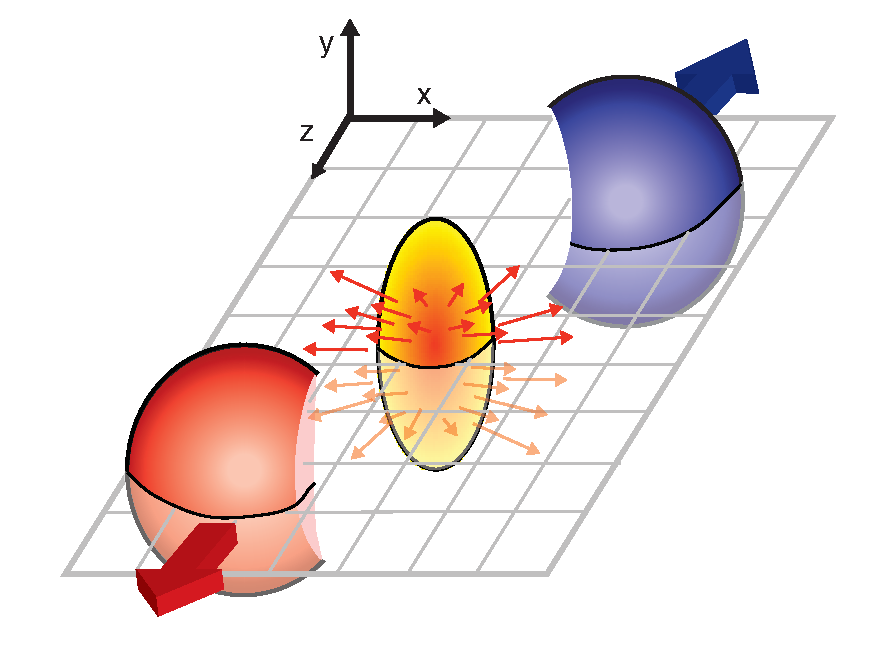
\includegraphics[width=4.5in]{figures/flow_elliptic_init_v4.pdf}
	  \caption{ \cite{}}\label{fig:}
	\end{figure}

\section{Calculations from the Spectral Fits}
\subsection{Assumptions of Particle Productions}
It is reasonable to assume that, at high energies, there should be roughly the same number of isospin states of a particle produced. 
	\begin{equation}\label{eqn:rapidityTransformation}
	E_{T} = 3E_{T}_\pi + 4E_{T}_\kappa + 4E_{T}_p + 2E_{T}_\lambda
	y' = y - y_{\beta}
	\end{equation}
 
\subsection{}
\subsection{}
\section{Uncertainties}
%\section{}
